\section{Logique}
\subsection{Division}
Afin de garder au maximum un code propre et lisible, 
et ainsi d'éviter d'avoir un fichier de 1000 lignes, 
j'ai décidé de le scinder en plusieurs parties. 
Ainsi les différents packages sont : 
\begin{itemize}
    \item Main 
    \item Menu (contient tout ce qui est relatif à un menu)
    \item Waiter (est ce que vous avez appelé "master" au sein des consignes)
    \item Coq 
    \item Intendant 
    \item Dispensers 
\end{itemize}

La logique respecte vos consignes, cependant, 
afin de mieux schématiser la situation, j'ai réalisé le schéma de la figure 2.

\subsection{Communication entre les acteurs}
Je suis parti du principe que nous allions reconstituer un restaurant classique.
Ainsi, nous avons le serveur (\textit{Waiter}) qui prend les commandes auprès des clients 
(nous donc) et qui transmet ces commandes à la cuisine, c'est à dire au chef. 
Ensuite le chef se charge de préparer chaque plat. C'est pourquoi nous avons la classe
\textit{Meal}, qui représente, pour chaque commande, sa préparation en cuisine. 
Le chef demande dans un premier temps un ingrédient de base à son intendant (\textit{Intendant}), 
puis demande aux commis de cuisines (\textit{Dispensers}) de lui ramener des ingrédients 
afin de compléter le plat. Toutes les communications entre le chef et ses délégués se font via une 
demande \textit{ask} de Akka. Seuls les communication entre le chef et son serveur se font via 
un \textit{tell}. 

\subsection{Améliorations de l'algorithme}
L'algorithme de sélection d'ingrédients (décrit dans le premier rapport, 
avec un système de calories et en fonction du type de repas et du sexe) n'est pas réellement 
amélioré. En effet, je préférais réaliser une implémentation propre du système d'acteur 
en gardant une architecture proche d'une cuisine plutôt que de m'attarder sur la sélection
d'ingrédient puisque, selon moi, cette partie était moins 
intéressante (de plus que je ne savais pas sur quoi me baser pour réaliser ma sélection d'ingrédients).
Cependant, avec cette nouvelle implémentation, nous retrouverons dans les plats préparés, des ingrédients 
contenant un minimum de sucre, de protéines et de gras tout en s'assurant que les calories totales ne sont 
pas dépassées en fonction du repas (déjeuner, diner ou souper).

Concernant les quantités, le fichier \textit{.csv} n'était pas fort fourni. C'est la raison pour laquelle,
si vous décidez de lancer 100 plats, vous n'aurez des quantités indiquées que pour très peu d'ingrédients (< 2\%).

\subsection{Remarques}
Je n'ai pas rédigé de commentaires (outre ceux indiquant les différentes
utilisations des méthodes propre à scala demandés) puisque un code se doit d'être compréhensible en le lisant
via les différents choix de nom de variables, de fonctions, etc.
De plus, pour un code susceptible d'évoluer dans le temps, les commentaires ne sont que trop rarement 
modifiés pour respecter ce qu'ils documentent.
Ainsi, j'espère que vous apprécierez mon effort de rendre le code le plus lisible et compréhensible possible
(j'ai nottament tenté de respecter les conventions de nommage propre à Scala).

J'ai nottament implémenté un moyen simple de tester plusieurs commandes à la fois 
(générées de façon aléatoire) afin de prouver que la coordination entre les différents acteurs 
fonctionnent. Il vous suffira de taper 2 au premier input demandé par le programme.
Pour avoir testé pour 25.000 plats à la fois, je n'ai pas relevé de problème. 
Cependant, pour une raison que je ne parviens pas à comprendre, si vous demander trop de commande, 
le chef commencera à recevoir de mauvaises réponses de la part de ses commis (sans pour autant crasher,
puisque la gestion des erreurs se fait correctement).

\vfill
\begin{figure}[H]
    \centering
    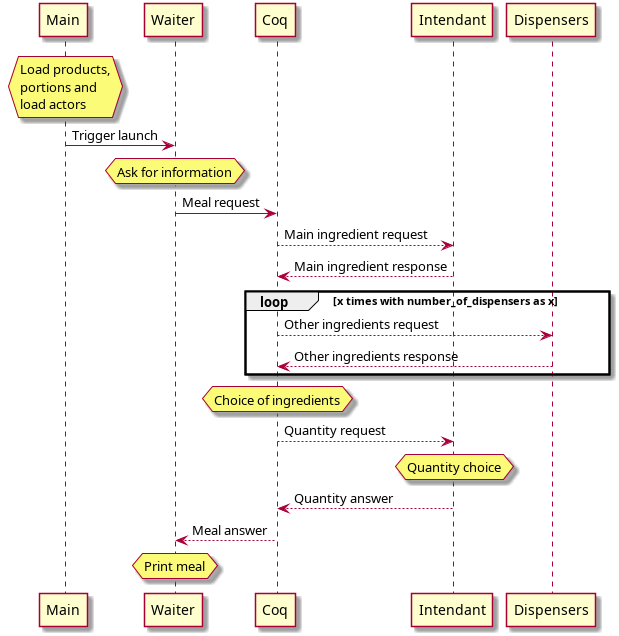
\includegraphics[width=0.8\textwidth]{parts/pics/diagram.png}
    \caption{Diagramme de séquence}
    \label{fig:my_label}
\end{figure}